\documentclass{standalone}
\usepackage{preset}
\begin{document}
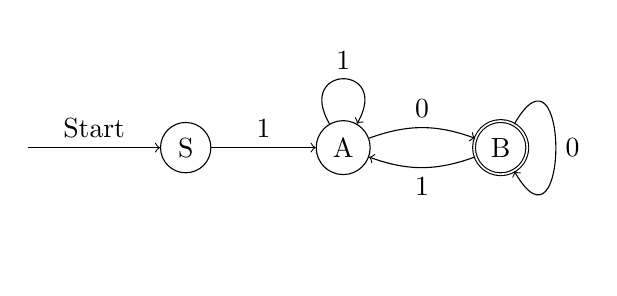
\begin{tikzpicture}[x=20mm,y=20mm]
	\node(S)at(0,0)[circle,draw]{S};
	\node(A)at(1,0)[circle,draw]{A};
	\node(B)at(2,0)[circle,draw,double]{B};
	\tikzset{every path/.style={->}}
	\draw(-1,0)--node[above]{Start}(S);
	\draw(S)--node[above]{1}(A);
	\draw(A)to[out=120,in=60,distance=25]node[above]{1}(A);
	\draw(A)to[out=20,in=160]node[above]{0}(B);
	\draw(B)to[out=-160,in=-20]node[below]{1}(A);
	\draw(B)to[out=60,in=-60,distance=40]node[right]{0}(B);
\end{tikzpicture}
\end{document}
